\section{Method}
\label{sec:method}

\subsection{Overview}
GraphPoint represents manipulation as interactions among 3D point entities and predicts future gripper points in the same geometric space.
As shown in Fig.~\ref{fig:framework}, language analysis, visual localization, and point tracking construct a task-conditioned entity graph, which a shared policy maps to a point trajectory and a subtask progress estimate.
For a multi-step instruction, the system instantiates this graph for each subtask and uses predicted progress to advance through the sequence.
The learned policy receives entity geometry and structured language conditions; color images are used by the perception front end.

\begin{figure*}[t]
\centering
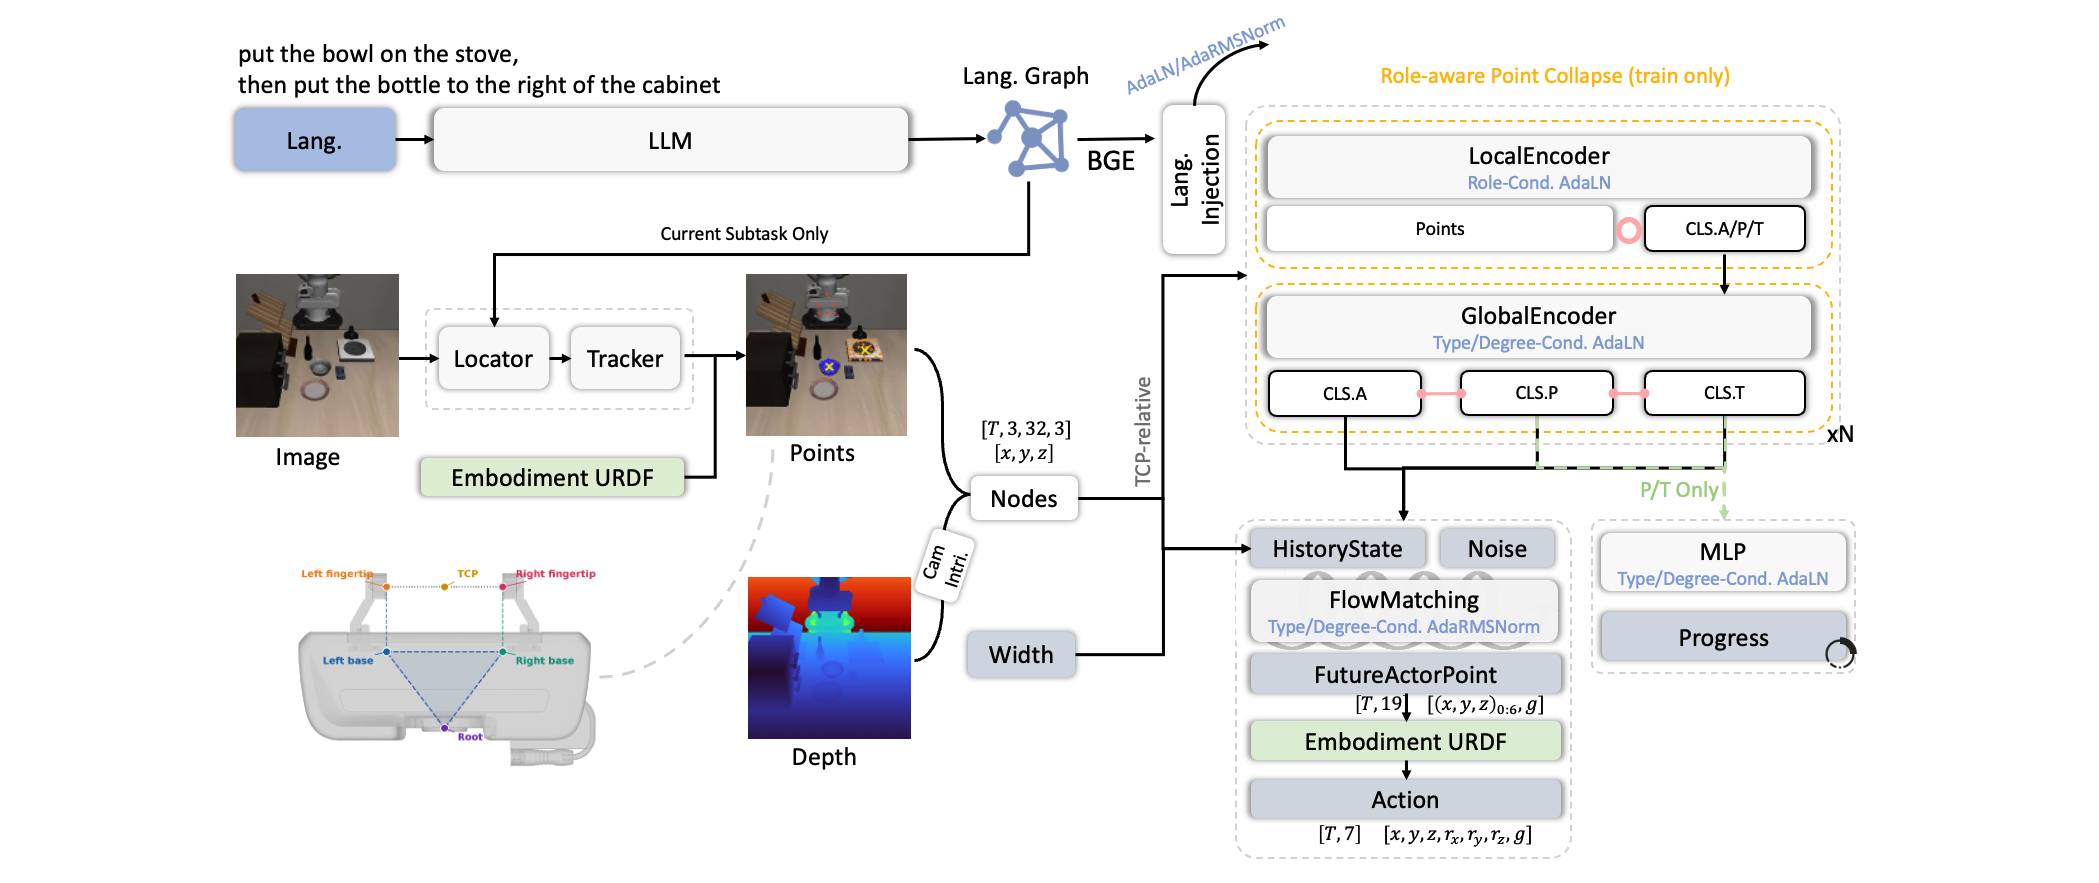
\includegraphics[width=\textwidth]{fig/main.png}
\caption{GraphPoint framework.
Language analysis identifies ordered subtasks and their semantic roles, while visual localization and tracking ground the relevant entities as 3D points.
The policy alternates local entity encoding with temporal graph attention, conditioned on roles, action types, and modifiers.
A flow decoder predicts future actor points and gripper commands, and a progress head supports subtask transitions.
Robot geometry converts predicted points into executable gripper poses.}
\label{fig:framework}
\end{figure*}
% Figure TODO: FutureActorPoint should have shape [H,19] for 6 XYZ points plus 1 gripper command, not [T,10].

\subsection{Task-to-Graph Construction}
\textbf{Semantic decomposition.}
A language model decomposes an instruction into ordered subtasks, each specified by an action type, a modifier, and entity roles.
The \emph{actor} $A$ denotes the gripper, the \emph{patient} $P$ denotes the manipulated object or part, and the \emph{target} $T$ denotes the reference entity.
For example, ``put the cheese to the right of the stove'' assigns cheese to $P$, stove to $T$, \emph{put} to the action type, and \emph{right} to the modifier.
Entity names guide visual grounding, whereas action types and modifiers are encoded separately using frozen BGE embeddings~\cite{xiao2024bge} and learned projections.
We denote their concatenation by the task condition $c$ and the learned embedding of role $r$ by $e_r$.
For readability, $c$ also denotes the version with separately normalized action and modifier embeddings used by the prediction heads.
Absent modifiers use a learned null embedding, and absent entities are masked.

\textbf{Grounded point entities.}
A pretrained vision-language locator identifies the requested objects or parts, and SAM~2~\cite{ravi2024sam2} produces masks from the localization prompts.
We sample 32 points per visual entity and track their image coordinates with TAPNext++~\cite{jung2026tapnextpp}.
Depth and camera intrinsics back-project these tracks into 3D.
The actor instead uses 6 keypoints computed from robot geometry and proprioception: the gripper root, TCP, 2 finger bases, and 2 fingertips.
We align all entities in camera coordinates and subtract the current TCP position from every point in the observation history and prediction horizon.
Thus, coordinates retain camera-axis orientation while sharing a translation origin at the current TCP.
This representation reduces dependence on absolute scene placement.
Actor points are padded with a validity mask, and coordinates are normalized using training-set quantiles.
The policy observes 10 frames, including the current frame.

\subsection{Role-Structured Entity Graph Encoder}
\textbf{Role-conditioned geometry and task-conditioned interaction.}
A shared point MLP embeds entity coordinates, with keypoint identity embeddings added for the actor.
Each entity at each observed time receives 4 learned CLS tokens to summarize its geometry.
The encoder alternates local encoding within each entity and global interaction among entity summaries:
\begin{equation}
\begin{aligned}
    (\widetilde C_r,F_r^{\ell+1})
       &=\operatorname{Local}_{\ell}(C_r^\ell,F_r^\ell;e_r),\\
    C^{\ell+1}
       &=\operatorname{Graph}_{\ell}(\{\widetilde C_r\}_{r\in\{A,P,T\}};c).
\end{aligned}
\label{eq:encoder}
\end{equation}
Here, $F_r$ and $C_r$ denote point features and CLS summaries, respectively, with observation-time indices omitted for clarity.
Local self-attention processes each entity and frame independently, conditioned on its role $e_r$.
Graph attention exchanges only CLS summaries across entities and observed times, conditioned on the action and modifier $c$.
Its connectivity follows the bidirectional chain $A\leftrightarrow P\leftrightarrow T$, with additional within-role temporal connections.
Direct actor--target attention is masked, so their interaction is mediated by the patient through successive layers.
This structure preserves separate entity summaries and encodes gripper--object and object--reference interactions.
Temporal rotary embeddings distinguish observation times.
After 8 layers, the current-time CLS summaries form memory $M_t$, incorporating both geometry and interaction history.

\textbf{Semantic injection.}
Both local and graph blocks contain attention and feed-forward sublayers, whose inputs are modulated through AdaLN:
\begin{equation}
    \operatorname{AdaLN}(h;q)
    =(1+\gamma(q))\odot\operatorname{LN}(h)+\beta(q).
\label{eq:adaln}
\end{equation}
The scale $\gamma$ and shift $\beta$ are learned functions of the condition, broadcast over tokens.
Local conditioning $q=e_r$ assigns roles to geometry; global conditioning $q=c$ distinguishes the instructed interaction, such as placing an object \emph{on} or to the \emph{right} of a target.

\textbf{Role-aware point collapse.}
During training, role-aware point collapse (RPC) independently collapses each patient or target point set with probability 0.05 to reduce dependence on detailed object shape.
For the patient, all points are replaced by the mean of the 4 points nearest to the TCP; for the target, they are replaced by the entity centroid.
This operation is applied consistently over the sampled temporal window, with anchors computed separately at each frame.
It preserves point counts and validity masks and leaves actor points and future action supervision unchanged.
The anchors retain the patient interaction region and target reference location while simplifying shape.

\subsection{Point-Trajectory Flow Policy}
We predict $H=10$ future steps, each containing 6 actor points and a scalar gripper command:
\begin{equation}
    Y=\{(X^A_{t+h},g_{t+h})\}_{h=1}^{H}.
\label{eq:point_trajectory}
\end{equation}
Here, $X^A_{t+h}$ contains actor coordinates relative to the current TCP, and $g_{t+h}$ is the open/close command.
Each step is represented by a 19-dimensional vector in point-wise $(x,y,z)$ order followed by the gripper command.
Representing actions as gripper points makes the predicted motion spatially comparable to the observed entities and encodes orientation through the arrangement of multiple points.

\textbf{Geometry- and language-conditioned decoding.}
A 6-layer Transformer models this trajectory with conditional flow matching~\cite{lipman2022flow}.
It embeds the observed actor history $U_t$ together with the noisy future trajectory $Z_\tau$ and predicts a velocity field:
\begin{equation}
    v_\theta=\operatorname{Decoder}_{\theta}(Z_\tau,U_t;M_t,c,\tau).
\label{eq:decoder}
\end{equation}
Each decoder layer uses self-attention to relate trajectory steps, cross-attention to retrieve entity geometry from $M_t$, and a feed-forward sublayer to update features.
Future tokens attend to both history and future, while history tokens cannot attend to future tokens.
Temporal rotary embeddings encode their relative times.
Action and modifier semantics enter every sublayer through AdaRMSNorm, following the scale-and-shift principle of Eq.~\eqref{eq:adaln}.
Separate mappings of the task condition $c$ and flow-time embedding are added to generate the scale, shift, and residual gate.
A final projection of the future tokens produces the point and gripper velocity predictions.

% Submit the benchmark figure early so it appears beside the benchmark introduction.
\begin{figure*}[!t]
    \centering
    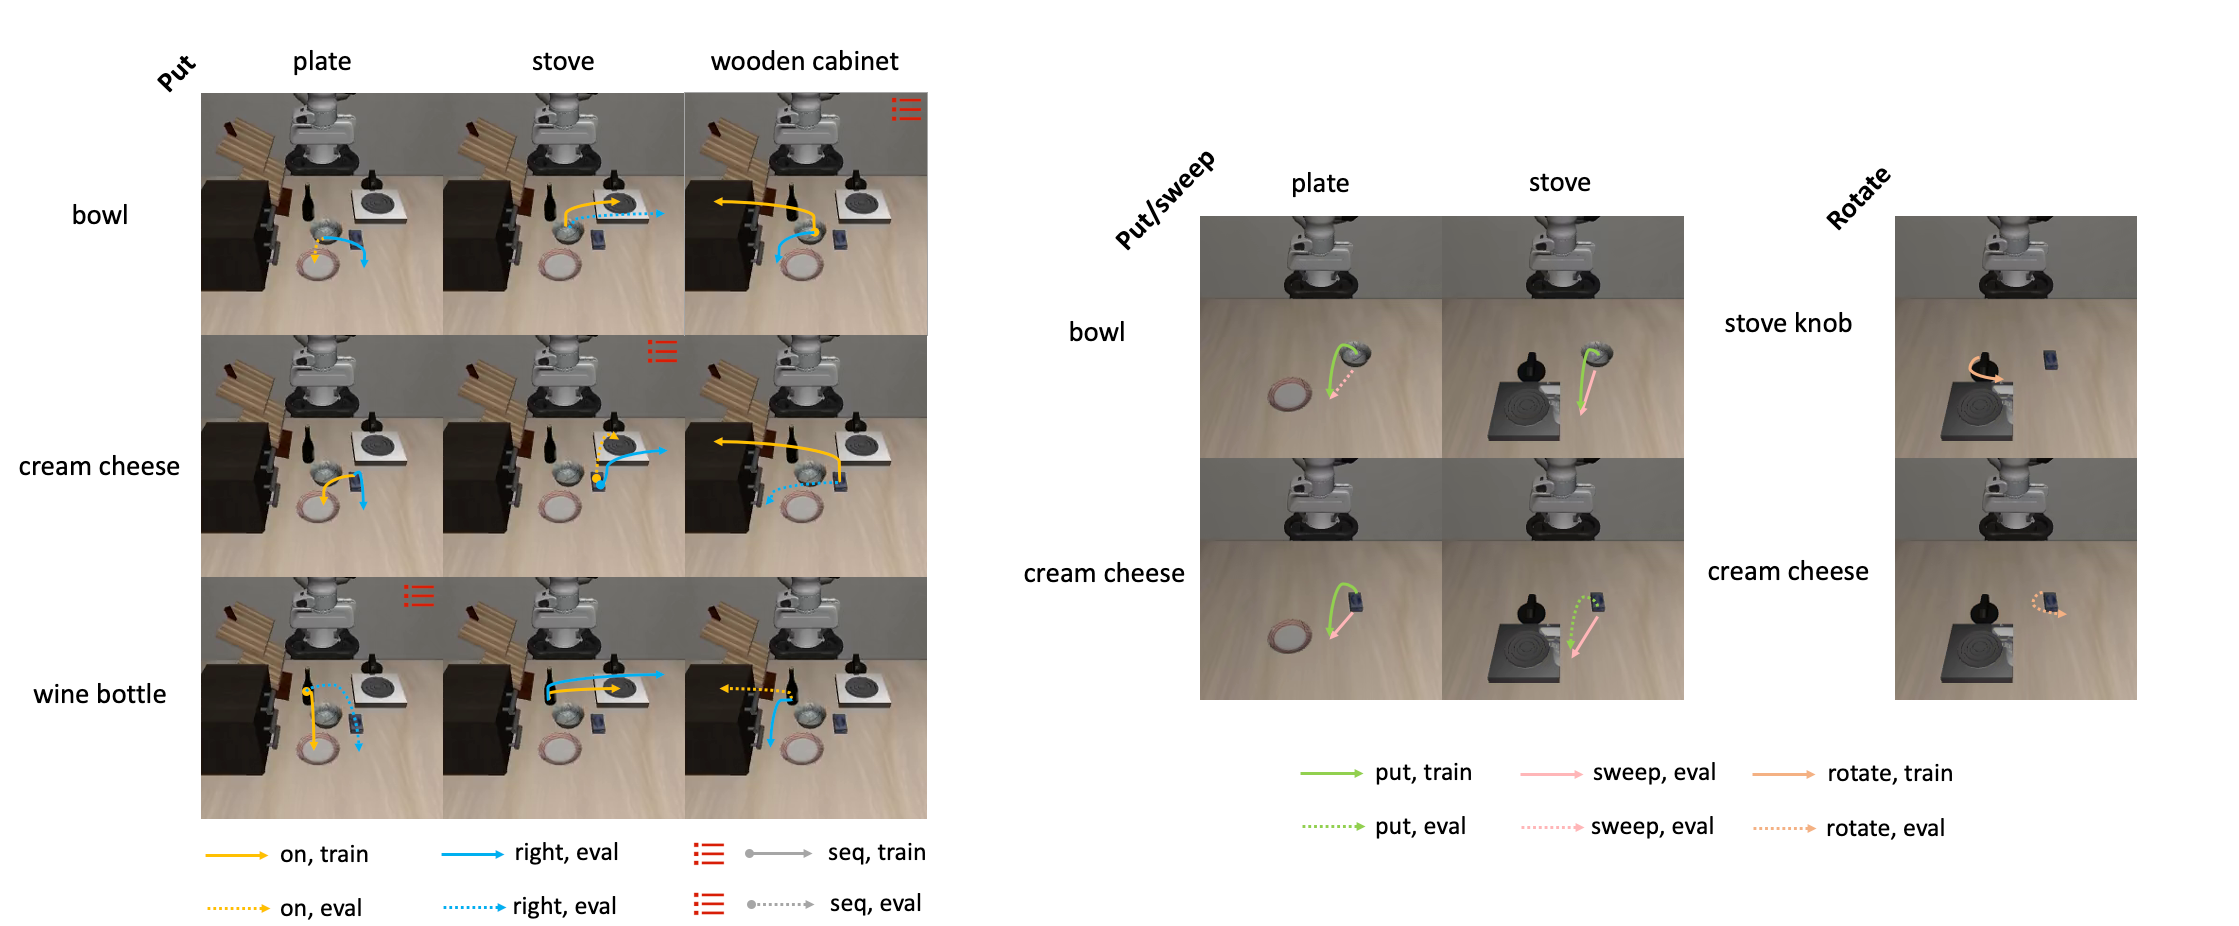
\includegraphics[width=\textwidth]{fig/benchmark.png}
    \caption{CoMani task construction and splits.
    Left: CoMani-Mod varies modifiers with a fixed put action.
    Center: CoMani-Act varies action types with a fixed right modifier.
    Right: CoMani-Seq composes atomic tasks from CoMani-Mod into 6 sequences of 3 steps, shown in 3 rows with execution proceeding from left to right.}
    \label{fig:benchmark}
\end{figure*}

\textbf{Training and execution.}
For a demonstrated trajectory $Y$ and Gaussian noise $\epsilon$, the flow objective is
\begin{equation}
\begin{aligned}
    Z_\tau&=(1-\tau)Y+\tau\epsilon,\\
    \mathcal L_{\mathrm{flow}}
       &=\mathbb E\!\left[\operatorname{MSE}(v_\theta,\epsilon-Y)\right],
\end{aligned}
\label{eq:flow}
\end{equation}
where the squared error is averaged over trajectory steps and output dimensions.
At inference, 10 Euler steps integrate from noise at $\tau=1$ to a trajectory at $\tau=0$.
After denormalization and restoring the TCP translation, we fit the robot's gripper keypoint template to each predicted point set using least-squares rigid alignment.
The template uses the observed gripper width, and the predicted gripper command is applied separately.
The recovered poses are transformed into the control frame and executed in a receding-horizon manner.

\subsection{Subtask Progress and Long-Horizon Composition}
The progress head estimates how far the active subtask has advanced from the current patient and target summaries:
\begin{equation}
    \hat{s}_t=\operatorname{Progress}_{\theta}(C_{t,P},C_{t,T};c).
\label{eq:progress}
\end{equation}
It uses a task-conditioned MLP with AdaLN and a sigmoid output, so the same geometry is evaluated under the active action and modifier.
The readout excludes direct actor summaries, although graph attention can propagate actor information into patient and target summaries.
Training targets increase linearly from 0 to 1 within each annotated subtask interval, and the complete objective is
\begin{equation}
    \mathcal{L}=\mathcal{L}_{\mathrm{flow}}+
    \operatorname{SmoothL1}(\hat{s}_t,s_t).
\end{equation}
At deployment, the planner advances when predicted progress exceeds a threshold for a consecutive window of policy calls.
We denote this learned transition rule as self-switching (SS).
Environment-based switching (ES) instead uses an environment-provided subtask completion signal to separate execution performance from learned transition timing.
On a transition, the system releases and lifts the gripper, selects the next subtask's entities and language conditions, and resets policy history.
The same atomic policy is reused throughout the sequence.
